\documentclass[a4paper]{article}
\usepackage{colortbl}
\usepackage[pages=all, color=black, position={current page.south}, placement=bottom, scale=1, opacity=1, vshift=5mm]{background}
\usepackage[margin=1in]{geometry} % full-width

% AMS Packages
\usepackage{amsmath}
\usepackage{amsthm}
\usepackage{amssymb}

% Unicode
\usepackage[utf8]{inputenc}
\usepackage{hyperref}
\hypersetup{
	unicode,
%	colorlinks,
%	breaklinks,
%	urlcolor=cyan, 
%	linkcolor=blue, 
	pdfauthor={Author One, Author Two, Author Three},
	pdftitle={A simple article template},
	pdfsubject={A simple article template},
	pdfkeywords={article, template, simple},
	pdfproducer={LaTeX},
	pdfcreator={pdflatex}
}

% Vietnamese
%\usepackage{vntex}

% Natbib
\usepackage[sort&compress,numbers,square]{natbib}
\bibliographystyle{mplainnat}

% Theorem, Lemma, etc
\theoremstyle{plain}
\newtheorem{theorem}{Theorem}
\newtheorem{corollary}[theorem]{Corollary}
\newtheorem{lemma}[theorem]{Lemma}
\newtheorem{claim}{Claim}[theorem]
\newtheorem{axiom}[theorem]{Axiom}
\newtheorem{conjecture}[theorem]{Conjecture}
\newtheorem{fact}[theorem]{Fact}
\newtheorem{hypothesis}[theorem]{Hypothesis}
\newtheorem{assumption}[theorem]{Assumption}
\newtheorem{proposition}[theorem]{Proposition}
\newtheorem{criterion}[theorem]{Criterion}
\theoremstyle{definition}
\newtheorem{definition}[theorem]{Definition}
\newtheorem{example}[theorem]{Example}
\newtheorem{remark}[theorem]{Remark}
\newtheorem{problem}[theorem]{Problem}
\newtheorem{principle}[theorem]{Principle}

\usepackage{graphicx, color}
\graphicspath{{fig/}}

%\usepackage[linesnumbered,ruled,vlined,commentsnumbered]{algorithm2e} % use algorithm2e for typesetting algorithms
\usepackage{algorithm, algpseudocode} % use algorithm and algorithmicx for typesetting algorithms
\usepackage{mathrsfs} % for \mathscr command
\usepackage{graphicx}
\usepackage{lipsum}

% Author info
\title{CSL2050 - Pattern Recognition and Machine Learning}
\author{
    \LARGE\textbf{Object Recognition - CIFAR10} \\
    \\ \\ \\ \\ \\
    \textbf{Team Member }\vspace{.5cm} \\
    Rohan Regar\vspace{} \\
    Arnava Srivastava \\
    Buddhav Garg \\
    Dheeraj Dhakar \\
    Harshit Barwar\\
    \\ \\
    \\ \\
}

\date{
        \\ \\
	 \\ \ \\%
	Anand Mishra \\ \texttt{Assistant Professor, Dept of CSE \\ \\ IIT Jodhpur}\\[2ex]%
%	\today
}


\begin{document}
	\maketitle
        \newpage
	\begin{abstract}
 The project aimed to optimize and enhance the performance of machine learning classifiers on the CIFAR-10 dataset, a well-known benchmark dataset for image classification. Various techniques were explored, including feature extraction using ResNet-50, Histogram of Oriented Gradients (HoG), and hyperparameter tuning for classification algorithms such as K-Nearest Neighbors (KNN), Decision Trees, and Naive Bayes.\\
The findings indicate that leveraging deep learning features, especially from models like ResNet-50, coupled with hyperparameter optimization, can substantially enhance the image classification performance on the CIFAR-10 dataset. The study underscores the significance of feature engineering and model tuning in achieving better results for image classification tasks.\\
	
		\noindent\textbf{Keywords:} Image Classification, CIFAR-10 Dataset, Machine Learning, ResNet-50, Hyperparameter Tuning.
	\end{abstract}

	\tableofcontents
        \newpage
	\section{Introduction}
    \hspace{.5cm}\textbf{Problem Statement:}\\
    In this project, we aimed to explore various machine learning techniques for image classification on the CIFAR-10 dataset. The CIFAR-10 dataset consists of 60,000 32x32 color images in 10 classes, with 6,000 images per class. Our objective was to build and evaluate different machine learning models to classify these images into their respective categories.\vspace{.5cm}

    \textbf{Major Findings:}
    \begin{itemize}
    \item Initial attempts with classical machine learning techniques like k-NN, decision trees, random forests, and Naive Bayes yielded moderate accuracy.
    \item Feature extraction using pretrained ResNet-50 CNN significantly improved classification accuracy, achieving up to 80%.
    \item Parameter optimization and failure case analysis further refined the models, providing insights into misclassifications.
    \end{itemize}\vspace{.5cm}

\textbf{Structure of Code File:}\\ 

\textbf{Data Preprocessing:}
\begin{itemize}
    \item Loading and visualizing the CIFAR-10 dataset.
    \item Data normalization and flattening.
\end{itemize}

\textbf{Testing Classical Machine Learning Models:}
\begin{itemize}
    \item KNN, Decision Trees, Random Forest, and Naive Bayes classifiers were trained and evaluated on the CIFAR-10 dataset.
\end{itemize}

\textbf{Techniques to Improve Accuracy:}
\begin{itemize}
    \item Linear Discriminant Analysis (LDA): Used to maximize class separation.
    \item Principal Component Analysis (PCA): Employed for dimensionality reduction.
    \item Feature Extraction Using ResNet-50.
    \item Histogram of Oriented Gradients (HOG): Feature extraction method to capture image gradients.
\end{itemize}

\textbf{Performance Comparison with Feature Extraction:}
\begin{itemize}
    \item Classical machine learning models were retrained using the features extracted by LDA, PCA, and HOG techniques.
    \item Failure case analysis using misclassification.

\end{itemize}

 \subsection{References}
 \begin{itemize}
     \item Utilized feature extraction code from professors Github Repo.\url{https://github.com/anandmishra22/PRML-Spring-2023/blob/main/Project/Reference_Codes/refCodes4PRMLProject.ipynb}
     \item Learned the basics to implement HoG from this page. \url{https://www.analyticsvidhya.com/blog/2019/09/feature-engineering-images-introduction-hog-feature-descriptor/}
     \item Understanding of ResNet-50 from following Link. \url{https://medium.com/@sharma.tanish096/detailed-explanation-of-residual-network-resnet50-cnn-model-106e0ab9fa9e}
     \item Hyperparameter Tuning from following link are used to understand while Implementaion. \url{https://www.anyscale.com/blog/what-is-hyperparameter-tuning}
 \end{itemize}
    
    
	\newpage
	

\section{Approach}

\textbf{Classical ML Techniques:}
We explored several classical machine learning techniques:
\begin{itemize}
    \item k-NN (k-Nearest Neighbors): We experimented with k-NN while optimizing parameters to find the optimal number of neighbors for classification.
    \item Decision Tree: Decision tree-based methods were used for classification tasks.
    \item Random Forest: Ensemble techniques like random forests were employed to improve classification accuracy by combining multiple decision trees.
    \item Naive Bayes: We implemented Naive Bayes, a probabilistic classifier commonly used in machine learning.
    \item SVM (Support Vector Machine): Model used for classification and regression tasks, aiming to find the optimal hyperplane that best separates data points into different classes
\end{itemize}

\textbf{Dimensionality Reduction:}
We applied Principal Component Analysis (PCA) and Linear Discriminant Analysis (LDA) to reduce the dimensionality of the feature space. However, no significant improvements were observed with these techniques.

\textbf{Feature Extraction using Pretrained CNN (ResNet-50):}
We utilized a pretrained Convolutional Neural Network (CNN) architecture, ResNet-50, to extract features from the images. Features were extracted from the last layer of the ResNet-50 model, capturing high-level image representations.

\textbf{Histogram of Oriented Gradients (HoG):}
We employed the Histogram of Oriented Gradients (HoG) technique as a feature descriptor to capture the local shape and edge information within the images. HoG features were computed to represent the distribution of gradient orientations in different image regions, providing valuable information for classification tasks.


\section{Experiments and Results}

\begin{enumerate}

\subsection{CIFAR-10 Dataset}

\item{Overview}
The CIFAR-10 dataset consists of 60,000 32x32 color images in 10 classes, with 6,000 images per class.

\item{Data Format}
The dataset is provided in a binary format, where each image is a 32x32 RGB image, resulting in a shape of (60000, 32, 32, 3).

\item{Reference}
The dataset and methodology followed are described in greater detail in the following paper: \url{https://www.cs.toronto.edu/~kriz/learning-features-2009-TR.pdf}.

\item{Loading Data}
The dataset can be loaded using the unpickle method to access the training and test sets separately.

\subsection{Data Preprocessing}


\item{Normalization}
Normalization is performed using min-max scaling to scale the pixel values from the range 0-255 to 0.0-1.0 (feature scaling). This is done because the pixel values in the RGB channels of the feature set range from 0-255.

\item{Flattening}
Flattening is typically done as traditional machine learning models require input in 2-D/tabular format.


\newpage
\subsection{Preliminary Tests}

\text{We apply KNN, Decision Tree, Random Forest, Naive Bayes, SVM, ANN and following are the }\\
\text{results of these Traditional Models}\\
\begin{table}[h!]
\centering
\caption{Performance metrics measures for classical techniques -}
\label{my-label}
\resizebox{15cm}{2.5cm}{
\begin{tabular}{|l|l|l|l|l|}
\hline
\rowcolor{gray!50} \textbf{MODELS} & \textbf{Accuracy} & \textbf{Precision} & \textbf{Recall} & \textbf{F1-score} \\ \hline
\rowcolor{lightgray!30} KNN             & 0.339             & 0.430              & 0.339           & 0.326             \\ \hline
\rowcolor{lightgray!30} Decision Tree   & 0.2673            & 0.267              & 0.2673          & 0.267             \\ \hline
\rowcolor{lightgray!30} Random Forest   & 0.472             & 0.468              & 0.472           & 0.470             \\ \hline
\rowcolor{lightgray!30} Naive Bayes     & 0.297             & 0.311              & 0.297           & 0.275             \\ \hline
\rowcolor{lightgray!30} SVM             & 0.544             & 0.542              & 0.544           & 0.542             \\ \hline
\rowcolor{lightgray!30} ANN             & 0.476             & 0.489              & 0.476          & 0.472             \\ \hline
\end{tabular}%

}

\end{table}\\
\vspace{.5cm}
\textbf{Resons for the failure of different Classical Machine Learning Models :}\\
\textbf{1. K-NN}
\begin{itemize}
    \item Curse of Dimensionality: CIFAR-10 images have a high dimensionality (32x32x3 = 3072 features). KNN struggles with high-dimensional data due to the curse of dimensionality.
    \item Pixel Values: RGB pixel values between 0 and 255 are treated as independent features. This approach doesn't capture spatial hierarchies and relationships between pixels.
\end{itemize}
\textbf{2. Decision Tree}
\begin{itemize}
    \item Overfitting: Decision trees can easily overfit to training data, especially with high-dimensional data like images.
    \item Lack of Feature Relationships: Decision trees make decisions based on individual features without considering the relationships between them, making it hard to capture complex patterns in images.
\end{itemize}
\textbf{3. Random Forest Classifier}
\begin{itemize}
    \item Complexity: Even though random forests can handle high-dimensional data better than decision trees, they might still struggle with capturing spatial hierarchies and intricate relationships in images.
    \item Ensemble of Weak Learners: Random forests are ensembles of decision trees, which might not be ideal for capturing the complexities of image data without deep feature extraction.
\end{itemize}
\textbf{4. Naive Bayes Classifier}
\begin{itemize}
    \item Independence Assumption: Naive Bayes assumes that features are independent, which is not the case for image data. Pixels in images are spatially correlated, and their relationships are crucial for classification.
    \item Continuous Features: Naive Bayes works well with categorical features but struggles with continuous features like pixel values in images.
\end{itemize}
\textbf{5. Support Vector Machine (SVM)}
\begin{itemize}
    \item High-Dimensional Data: SVMs perform well in low to medium-dimensional spaces but can become computationally expensive and inefficient in high-dimensional spaces like the CIFAR-10 dataset (32x32x3 = 3072 features).
    \item Linear Separability: SVM aims to find the hyperplane that best separates the data into different classes. In the case of CIFAR-10 images, the data might not be linearly separable in the feature space defined by raw pixel values. This can lead to suboptimal decision boundaries and reduced classification accuracy.
    \item Kernel Selection: While SVM can utilize various kernels to handle non-linear data, selecting an appropriate kernel and tuning its parameters can be challenging and computationally expensive for high-dimensional image data.
\end{itemize}

\subsection{Methods Used to Improve Performance }
\textbf{Dimensionality Reduction:} Techniques like PCA and LDA can be applied to reduce the dimensionality of the data, making it easier for classical ML models to handle.\\
\textbf{Deep Learning and CNNs:} Deep learning models like Convolutional Neural Networks (CNNs) are well-suited for image classification tasks. They can automatically learn hierarchical features from images, capturing spatial relationships and patterns.\\
\textbf{Feature Engineering:} Instead of using raw pixel values, feature engineering techniques like histogram of oriented gradients (HoG), or using pretrained models for feature extraction can be beneficial.\\
\textbf{Hyperparameter Tuning:} Optimize the hyperparameters of the classical ML models to find the best configuration for the CIFAR-10 dataset.\\

\subsubsection{Performance After Dimensionality Reduction }
After applying dimensionality reduction techniques like LDA (Linear Discriminant Analysis) and PCA (Principal Component Analysis), the performance of the machine learning models exhibited varied outcomes. Notably, there was a slight improvement in accuracy for the Naive Bayes classifier. However, the accuracy decreased for the Random Forest and SVM classifiers. The performance of the Decision Tree and K-Nearest Neighbors (KNN) classifiers remained relatively unchanged.
\begin{table}[h!]
\centering
\caption{Performance metrics measures after performing PCA -}
\label{my-label}
\resizebox{15cm}{2.5cm}{
\begin{tabular}{|l|l|l|l|l|}
\hline
\rowcolor{gray!50} \textbf{MODELS} & \textbf{Accuracy} & \textbf{Precision} & \textbf{Recall} & \textbf{F1-Score} \\ \hline
\rowcolor{lightgray!30} KNN       & 0.362       & 0.446       & 0.362       &0.354          \\ \hline
\rowcolor{lightgray!30} Decision Tree  & 0.257      & 0.257       & 0.257     &0.257         \\ \hline
\rowcolor{lightgray!30} Random Forest  & 0.434       & 0.429       & 0.434      &0.430           \\ \hline
\rowcolor{lightgray!30} Naive Bayes   & 0.312       & 0.333       & 0.312       &0.299           \\ \hline
\rowcolor{lightgray!30} SVM       & 0.470       & 0.506       & 0.470          &0.478  \\ \hline
\rowcolor{lightgray!30} ANN       & 0.520       & 0.520       & 0.520          &0.514  \\ \hline
\end{tabular}
}
\end{table}
\begin{table}[h!]
\centering
\caption{Performance metrics measures after performing LDA -}
\label{my-label}
\resizebox{15cm}{2cm}{
\begin{tabular}{|l|l|l|l|}
\hline
\rowcolor{gray!50} \textbf{MODELS} & \textbf{Accuracy} & \textbf{Precision} & \textbf{Recall} \\ \hline
\rowcolor{lightgray!30} KNN       & 0.329       & 0.334       & 0.329           \\ \hline
\rowcolor{lightgray!30} Decision Tree  & 0.278      & 0.278       & 0.278         \\ \hline
\rowcolor{lightgray!30} Random Forest  & 0.369       & 0.368       & 0.369           \\ \hline
\rowcolor{lightgray!30} Naive Bayes   & 0.365       & 0.366       & 0.365           \\ \hline
\rowcolor{lightgray!30} SVM       & 0.373       & 0.373       & 0.373            \\ \hline
\end{tabular}
}
\end{table}\\

\begin{itemize}
    \item \textbf{Improvement:} LDA and PCA might have enhanced the feature separability, making the data more discriminative, which could have benefited the Naive Bayes classifier that assumes feature independence.
    \item \textbf{Decrease in Accuracy:}
    \begin{itemize}
        \item Loss of Information: Dimensionality reduction techniques like LDA and PCA might have resulted in the loss of some discriminative information crucial for the Random Forest and SVM classifiers, affecting their performance negatively.
        \item Complexity Reduction: Random Forest and SVM, being inherently capable of handling high-dimensional data, might not benefit significantly from dimensionality reduction and could even suffer due to reduced feature space.
    \end{itemize}

\end{itemize}
\vspace{0.5cm}
\subsubsection{Performance After Using HoG }
HoG is a feature descriptor that captures the distribution of gradients (edge orientations) in an image. It is used primarily in computer vision tasks for object detection and image classification.\\

Key Parameters:
\begin{itemize}
    \item Orientations: Number of gradient orientations to consider (e.g., 9 orientations).
    \item Pixels per Cell: Size of the cell in pixels (e.g., 8x8 pixels).
    \item Cells per Block: Number of cells in each block (e.g., 2x2 cells).
\end{itemize}
We have used the template code provided for applying HoG.
\begin{table}[h!]
\centering
\caption{Performance metrics measures after HoG -}
\label{my-label}
\resizebox{15cm}{2cm}{
\begin{tabular}{|l|l|l|l|l|}
\hline
\rowcolor{gray!50} \textbf{MODELS} & \textbf{Accuracy} & \textbf{Precision} & \textbf{Recall} & \textbf{F1-score} \\ \hline
\rowcolor{lightgray!30} KNN             & 0.523             & 0.572              & 0.524           & 0.518             \\ \hline
\rowcolor{lightgray!30} Decision Tree   & 0.279            & 0.281              & 0.279          & 0.280             \\ \hline
\rowcolor{lightgray!30} Random Forest   & 0.521             & 0.518              & 0.521           & 0.516             \\ \hline
\rowcolor{lightgray!30} Naive Bayes     & 0.458             & 0.466              & 0.458           & 0.454             \\ \hline
\rowcolor{lightgray!30} SVM             & 0.632             & 0.632              & 0.632            & 0.631           \\ \hline
\rowcolor{lightgray!30} ANN             & 0.479             & 0.479              & 0.470            & 0.471           \\ \hline
\end{tabular}%
}
\end{table}
\begin{itemize}
    \item Improved Accuracy: The classifiers trained on HoG features exhibited improved accuracy compared to models trained on raw pixel values, albeit not as high as those trained on ResNet features.
    \item Enhanced Feature Representation: HoG captures texture and shape information, which might be beneficial for distinguishing between different CIFAR-10 classes compared to raw pixel values.
    \item It may not capture the intricate details and relationships present in the data as effectively as a deep neural network like ResNet.
\end{itemize}

\vspace{0.5cm}

\subsubsection{Performance After Using ResNet-50 }
\begin{itemize}
    \item ResNet, which stands for Residual Network, is a type of deep neural network architecture that was introduced to address the problem of vanishing gradients in very deep neural networks. 
    \item It introduced the concept of residual learning to CNN architectures, and has a deep architecture making it relevant for tasks like image classification, object detection, and image segmentation.
    \item Transfer learning - We have used the template code provided for feature extraction from the last layer of a pre-trained ResNet-50 model.
\end{itemize}
After extracting features from the pre-trained ResNet-50 model and applying classical machine learning techniques, a significant improvement in accuracy was observed across multiple classifiers.\\

\begin{table}[h!]
\centering
\caption{Performance metrics measures after ResNet-50 -}
\label{my-label}
\resizebox{15cm}{2cm}{
\begin{tabular}{|l|l|l|l|l|}
\hline
\rowcolor{gray!50} \textbf{MODELS} & \textbf{Accuracy} & \textbf{Precision} & \textbf{Recall} & \textbf{F1-score} \\ \hline
\rowcolor{lightgray!30} KNN             & 0.841             & 0.844              & 0.841           & 0.840             \\ \hline
\rowcolor{lightgray!30} Decision Tree   & 0.646            & 0.647              & 0.646          & 0.646             \\ \hline
\rowcolor{lightgray!30} Random Forest   & 0.811             & 0.815              & 0.811           & 0.811             \\ \hline
\rowcolor{lightgray!30} Naive Bayes     & 0.792             & 0.794              & 0.792           & 0.791             \\ \hline
\rowcolor{lightgray!30} SVM             & 0.898             &               &            &            \\ \hline
\rowcolor{lightgray!30} Naive Bayes     & 0.878             & 0.878              & 0.878           & 0.880             \\ \hline
\end{tabular}%
}
\end{table}

\textbf{Improved accuracy: }The reason is simple - the features extracted from ResNet-50 are rich and high-dimensional, capturing intricate patterns and representations from the images. This solves the primary problem of capturing spatial correlations of the pixels, faced by the classical models.

\vspace{0.5cm}

\subsubsection{Hyperparameter Tuning}
While applying a pre-trained model like ResNet-50 is a powerful approach for the Cifar-10 dataset, there's still room for improvement through hyperparameter tuning on the final classification layer. Hyperparameter tuning is a crucial step in optimizing the performance of machine learning models. It involves selecting the best hyperparameters that govern the learning process of the model to achieve improved accuracy and generalization on unseen data.\\

\textbf{K-Nearest Neighbors (KNN)}
\begin{itemize}
    \item By varying the number of neighbors (k), the accuracy of the KNN classifier was evaluated.
    \item The optimal value of k was determined using a range of k values from 3 to 19.
    \item The accuracy plot displayed the performance of the KNN classifier for each k value, with a peak accuracy achieved at the best k value.
    \item\textbf{Best k value = 13}
\end{itemize}
\begin{figure}[h]
    \centering
    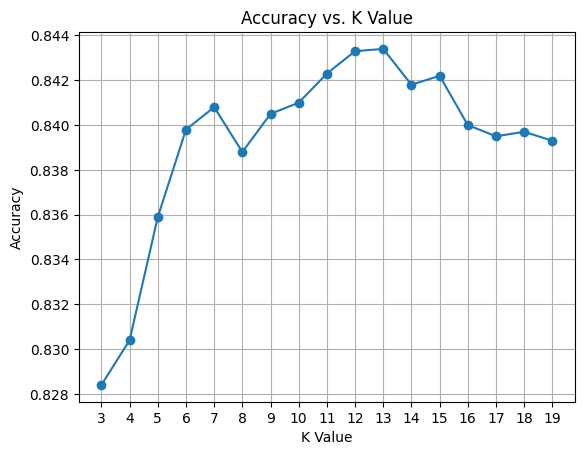
\includegraphics[width=0.5\textwidth]{download.png}
    \caption{Accuracy Plot for different values of k}
\end{figure}
\vspace{1cm}
\textbf{Decision Tree}
\begin{itemize}
    \item Two different criteria, "gini" and "entropy", were explored to split the nodes of the Decision Tree.
    \item Further hyperparameter tuning was conducted by setting constraints on the maximum depth of the tree, minimum samples leaf, and minimum samples split.
    \item Best parameter found from the grid 
    \begin{itemize}
        \item Max\textunderscore depth : [8,10 , 12],
        \item Min\textunderscore samples\textunderscore leaf : [8 ,10 ,12]
        \item Min\textunderscore samples\textunderscore split : [13,15,17] 
    \end{itemize}


  

    \item\textbf{The Decision Tree classifier achieved the highest accuracy when the criterion was set to "entropy" with a maximum depth of 10, minimum samples leaf of 10, and minimum samples split of 15.}
\end{itemize}

\textbf{Naive Bayes}
\begin{itemize}
    \item The \textbf{Multinomial} Naive Bayes classifier was optimized by tuning the alpha parameter, which represents the smoothing parameter.
    \item Grid Search Cross Validation was employed to find the optimal alpha value.
    \item The best alpha value obtained was 2.0, which resulted in an accuracy of 0.7915.
    \item The \textbf{Gaussian} Naive Bayes classifier was optimized by tuning the var\textunderscore smoothing parameter, which adds a fraction of the largest variance of all features to variances for calculation stability.
    \item The best hyperparameters found for Gaussian Naive Bayes were {'var\textunderscore smoothing': 1e-09} and accuracy achieved was 0.7948.
\end{itemize}

\textbf{Support Vector Machine (SVM)}
\begin{itemize}
    \item The SVM classifier was fine-tuned by exploring different combinations of hyperparameters such as C, gamma, and kernel.
    \item Grid Search Cross Validation was utilized to identify the optimal hyperparameters.
    \item The best hyperparameters found were {'C': 2, 'gamma': 'scale', 'kernel': 'rbf'}, with an accuracy score of 0.891 and the best score of 0.896.
\end{itemize}
\vspace{0.5cm}

\begin{table}[h!]
\centering
\caption{\textbf{Results of Accuracy After Hyperparameter Tuning}}
\label{my-label}
\resizebox{7.5cm}{1.5cm}{
\begin{tabular}{|l|l|}
\hline
\rowcolor{gray!50} \textbf{MODELS} & \textbf{Accuracy}  \\ \hline
\rowcolor{lightgray!30} KNN             & 0.843          \\ \hline
\rowcolor{lightgray!30} Decision Tree   & 0.663             \\ \hline
\rowcolor{lightgray!30} Naive Bayes     & 0.795             \\ \hline
\rowcolor{lightgray!30} SVM             & 0.891          \\ \hline

\end{tabular}%
}
\end{table}
\newpage
\subsection{Misclassification Results}
After evaluating the performance of various machine learning models, it's crucial to understand where these models are failing. Misclassification analysis provides insights into the specific classes that are often confused with each other by the models.
\begin{figure}[h]
    \centering
    \begin{minipage}{0.45\textwidth}
        \centering
        \caption{k-NN}
        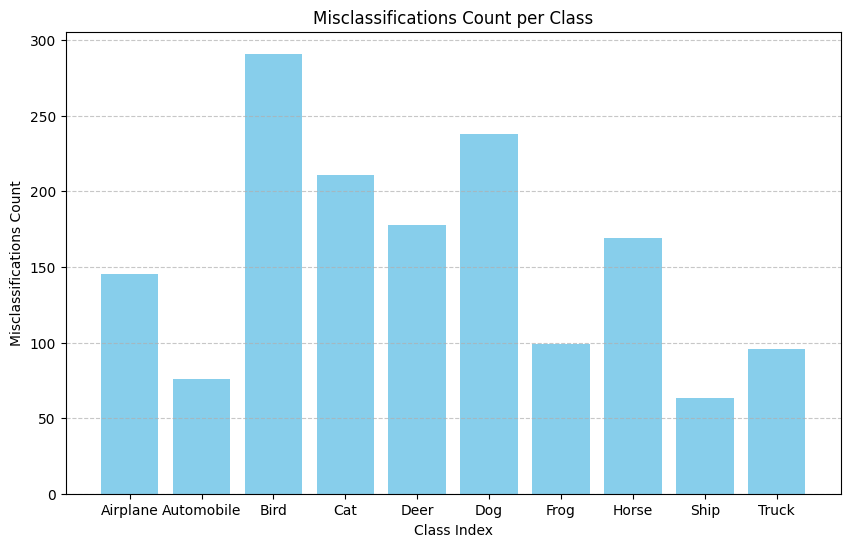
\includegraphics[width=\linewidth]{KNN.png}
    \end{minipage}\hfill
    \begin{minipage}{0.45\textwidth}
        \centering
        \caption{Decision Tree}
        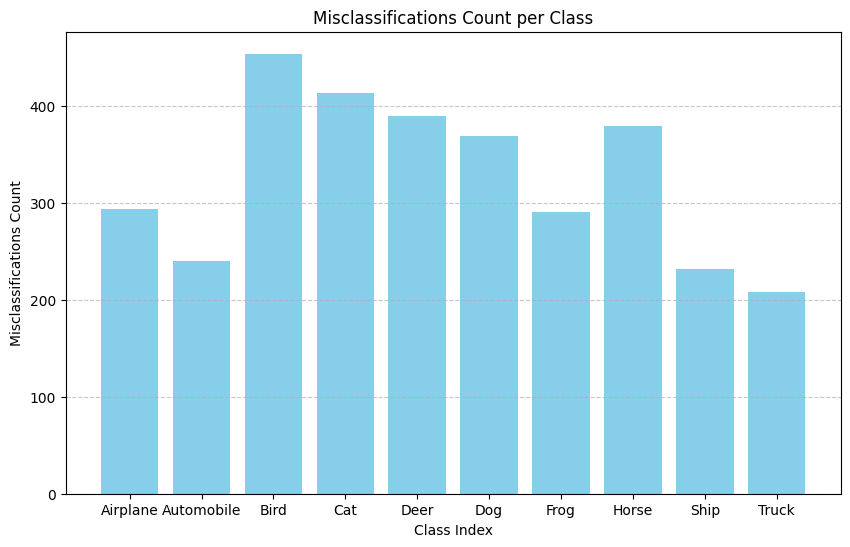
\includegraphics[width=\linewidth]{Decision Tree.png}
    \end{minipage}

    \begin{minipage}{0.45\textwidth}
        \centering
        \caption{Random Forest}
        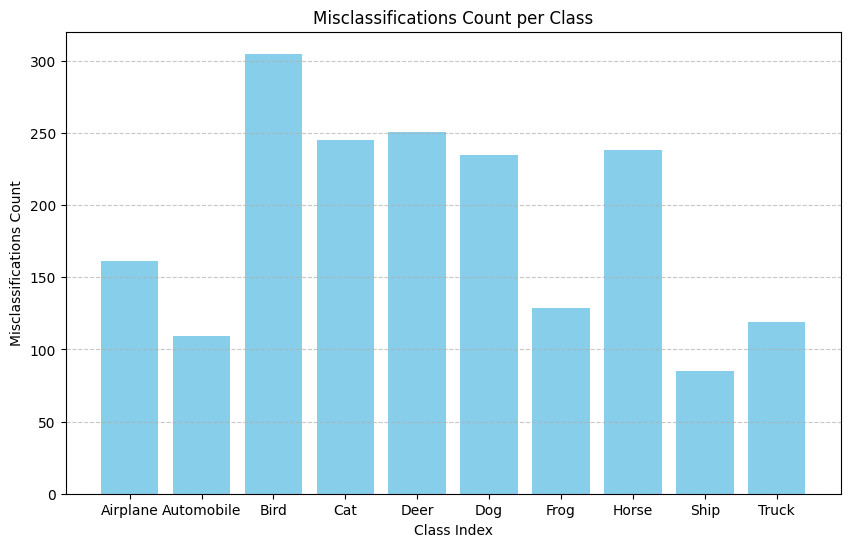
\includegraphics[width=\linewidth]{Random.png}
    \end{minipage}\hfill
    \begin{minipage}{0.45\textwidth}
        \centering
        \caption{Naive Bayes}
        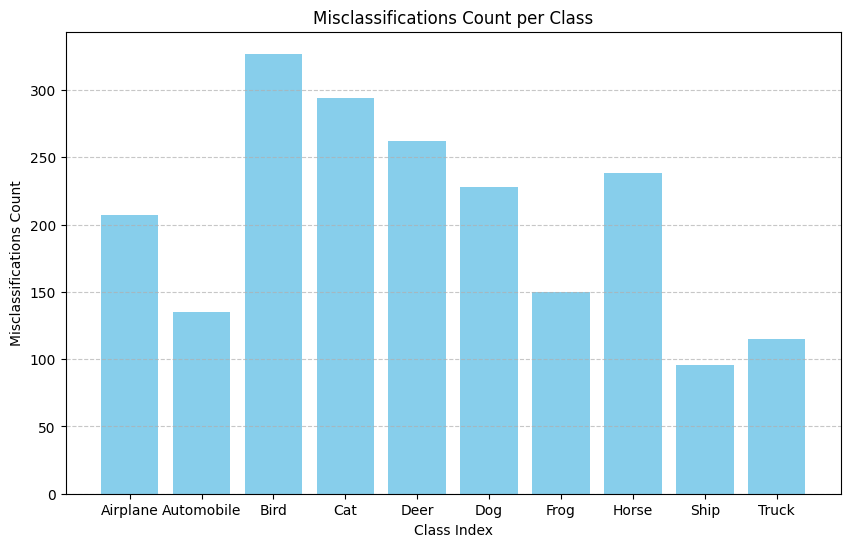
\includegraphics[width=\linewidth]{Naive Bayes.png}
    \end{minipage}
    \begin{minipage}{0.45\textwidth}
        \centering
        \caption{SVM}
        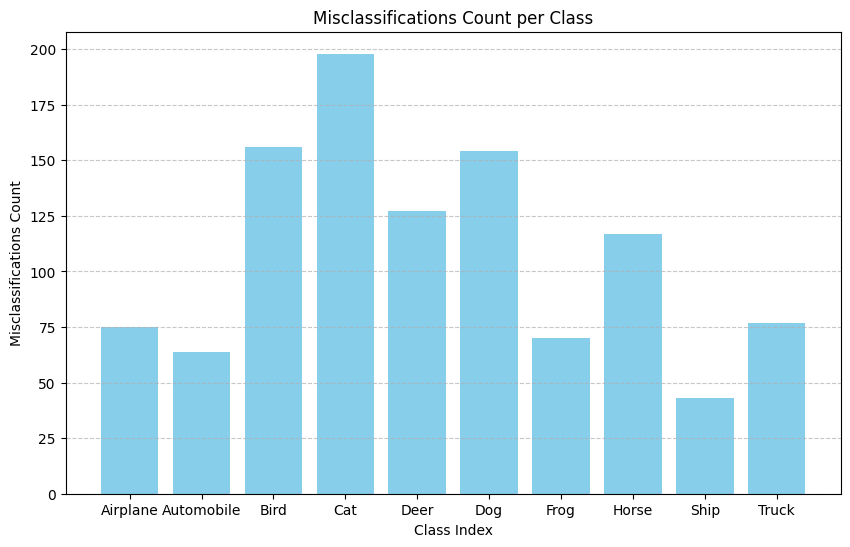
\includegraphics[width=\linewidth]{SVM.png}
    \end{minipage}\hfill
    \begin{minipage}{0.45\textwidth}
        \centering
        \caption{ANN}
        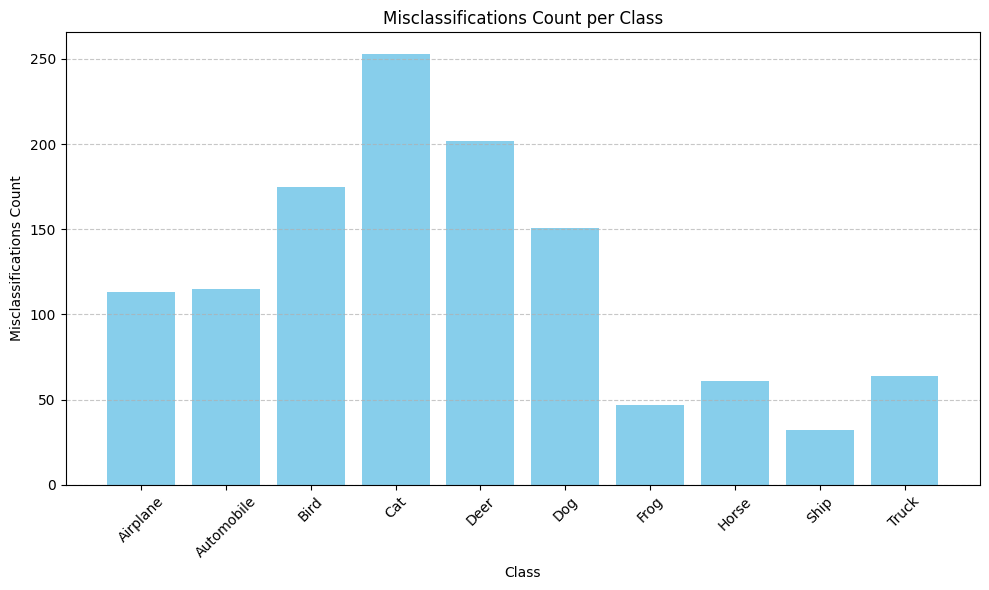
\includegraphics[width=\linewidth]{ANN.png}
    \end{minipage}
    \vspace{0.5cm}
\end{figure}\\
\textbf{Inferences:}
\begin{itemize}
    \item Uniform Misclassifications: Models like Decision Tree and Random Forest seem to generalize well across various classes but might benefit from more nuanced feature engineering or deeper architectures to capture intricate class differences.
    \item Specific Confusions: Models like Naive Bayes and SVM show specific pairs of classes where confusion is more frequent. This indicates the need for targeted improvements in feature extraction or model architecture to resolve these issues.
    \item Balanced Misclassifications: KNN and ANN shows a balanced misclassification pattern, suggesting a more holistic understanding of the data. 
\end{itemize}
\end{enumerate}


	\newpage
	
	
	\section{Summary}
	\label{sec:app}
	The report investigates image classification on the CIFAR-10 dataset using classical machine learning techniques and advanced methods like feature extraction with pretrained CNNs. Initially, traditional models like k-NN, decision trees, and random forests yielded moderate accuracy. However, feature extraction with ResNet-50 significantly improved classification accuracy to 0.80. Attempts to improve classical models through dimensionality reduction and feature engineering had mixed results, with slight improvements for some models but decreased accuracy for others. Histogram of Oriented Gradients (HoG) showed promise, albeit not as effective as deep learning methods. Finally, hyperparameter tuning further improved accuracy across various classifiers. Misclassification analysis highlighted areas for improvement, suggesting the need for more nuanced feature engineering and model architecture adjustments. Overall, leveraging deep learning techniques like ResNet-50 for feature extraction proved most effective in enhancing classification accuracy on the CIFAR-10 dataset.\\
 
 \textbf{Future Prospects}\\
As we delve deeper into the intricacies of the CIFAR-10 dataset, there are several avenues to explore for improving model performance:
\begin{itemize}
    \item Advanced Feature Engineering: Techniques like HoG and deep feature extraction (e.g., from pre-trained models like ResNet) have shown promise. Exploring more advanced feature engineering methods tailored to image data could yield significant improvements.
    \item Ensemble Methods: Combining the strengths of multiple models through ensemble methods can often lead to better generalization and reduced overfitting. Techniques like stacking or boosting could be explored.
    \item Neural Network Architectures: Experimenting with more complex neural network architectures, including convolutional neural networks (CNNs), can help in capturing intricate patterns in image data, potentially improving accuracy and reducing misclassifications.
\end{itemize}

	
\bibliographystyle{plain} % Specify the bibliography style
\bibliography{ref.bib} % Specify the BibTeX file containing references
	
	\appendix
	
	\section{Contribution of each member}
	\label{sec:contribution}
	\begin{enumerate}
	\item Rohan Regar: Implemented various classifier, conducted        analysis of performance, ideas in ResNet-50,HoG and some            parameter tuning. 
        \item Arnava Srivastava: Implemented failure case analysis of all models. Prepared presentation and youtube Video.
        \item Dheeraj Dhakar: Implemented dimensionality Reduction and its analysis. Prepared the project page for overall idea of project.
	\item Buddhav garg: Implemented feature extraction using HoG. Prepared the final report on LaTex.
	\item Harshit Barwar: Performed dataset analysis, pre-testing using classical ML models.
	\end{enumerate}
    	
	
\end{document}